% ----------------------------------------------------------------------------------------\
% ---------------------------------------------------------------------------------------\
% --------------------------------------------------------------------------------------\
\section{Investigación}
% ----------------------------------------------------------------------------------------\
% ---------------------------------------------------------------------------------------\
% Investiga y escribe un breve resumen sobre los algoritmos 
%  SVM (Support Vector Machine),
%  Decision Tree 
%  Random Forest.
% --------------------------------------------------------------------------------------\

% ----------------------------------------------------------------------------------------\
% ---------------------------------------------------------------------------------------\
\subsection{Algoritmos de aprendizaje supervisados}
% ----------------------------------------------------------------------------------------\
% ---------------------------------------------------------------------------------------\

Los algoritmos de aprendizaje supervisado experimentan un conjunto de datos que contiene 
características, pero cada ejemplo también está asociado con una etiqueta u objetivo. 
Por ejemplo, el conjunto de datos de Iris está anotado con la especie de cada planta de iris. 
Un algoritmo de aprendizaje supervisado puede estudiar el conjunto de datos de Iris y aprender 
a clasificar las plantas de iris en tres especies diferentes según sus mediciones.
\cite{Goodfellow-et-al-2016}\\ 

Es decir aprenden a asociar alguna entrada con alguna salida, dado un conjunto de entrenamiento 
de ejemplos de entradas $x$ y salidas $y$. En muchos casos, los resultados y pueden ser difíciles 
de recopilar automáticamente y deben ser proporcionados por un \textit{supervisor} humano, pero 
el término aún se aplica incluso cuando los objetivos establecidos de capacitación se 
recopilaron automáticamente.\cite{Goodfellow-et-al-2016}\\ 

Brevemente el contraste con los algoritmos de aprendizaje no supervisados experimentan un 
conjunto de datos que contiene muchas características y luego aprenden propiedades útiles de 
la estructura de este conjunto de datos. En el contexto del aprendizaje profundo, generalmente 
queremos aprender la distribución de probabilidad completa que generó un conjunto de datos, ya 
sea explícitamente como en la estimación de densidad o implícitamente para tareas como síntesis 
o eliminación de ruido. Algunos otros algoritmos de aprendizaje no supervisados desempeñan otras 
funciones, como el clustering, que consiste en dividir el conjunto de datos en grupos de 
ejemplos similares.\cite{Goodfellow-et-al-2016}\\


% ----------------------------------------------------------------------------------------\
% ---------------------------------------------------------------------------------------\
\subsection{Support Vector Machine}
% ----------------------------------------------------------------------------------------\
% ---------------------------------------------------------------------------------------\

Uno de los enfoques más influyentes para el aprendizaje supervisado es la máquina de vectores 
de soporte. Este modelo es similar a la regresión logística en el sentido de que está 
impulsado por una función lineal $w^{\intercal} x + b$. A diferencia de la regresión logística, 
la máquina de vectores de soporte no proporciona probabilidades, sino que solo emite una 
identidad de clase. La SVM predice que la clase positiva está presente cuando 
$w^{\intercal} x + b$ es positivo. De manera similar, predice que la clase negativa está 
presente cuando $w^{\intercal} x + b$ es negativo.\cite{Goodfellow-et-al-2016} \\ 

Una máquina de vectores de soporte (SVM) es un modelo de aprendizaje automático potente y 
versátil, capaz de realizar clasificación, regresión e incluso detección de novedades 
lineales o no lineales. Las SVM brillan con conjuntos de datos no lineales de tamaño pequeño 
y mediano (es decir, de cientos a miles de instancias), especialmente para tareas de 
clasificación. Sin embargo, como verá, no se adaptan muy bien a conjuntos de datos 
muy grandes. \cite{géron2022hands}\\ 


La idea fundamental detrás de las máquinas de vectores de soporte (SVM) es encontrar el 
hiperplano que mejor separa dos clases en un espacio de características, maximizando el 
margen entre las instancias de entrenamiento más cercanas a él. En términos simples, busca 
la mejor \textit{avenida} que divide dos grupos de puntos en un espacio multidimensional.\\

Por ejemplo, para la tarea de los correos electrónicos, clasificarlos como spam o no spam, 
tenemos un conjunto de datos con correos etiquetados y cada correo tiene características 
como la frecuencia de ciertas palabras clave, la longitud del mensaje, etc. Utilizando SVM, 
el algoritmo busca un hiperplano en este espacio de características que separe claramente 
los correos de spam de los correos legítimos. El margen entre este hiperplano y las 
instancias más cercanas de cada clase es maximizado, lo que ayuda a mejorar la capacidad de 
generalización del modelo.\\

\begin{center}
    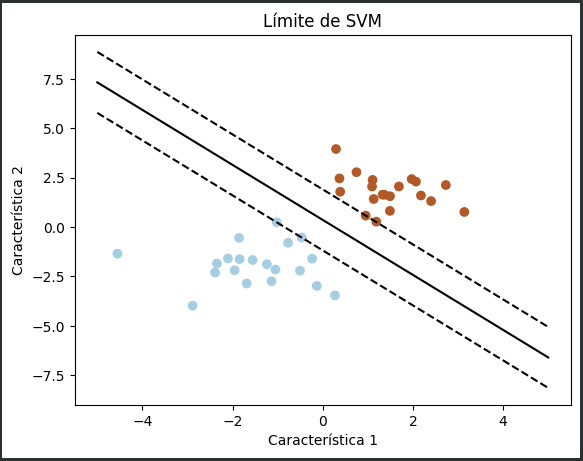
\includegraphics[scale = .5]{IMA/limiteSVM.png}
\end{center}

% ----------------------------------------------------------------------------------------\
% ---------------------------------------------------------------------------------------\
\subsection{Decision Tree}
% ----------------------------------------------------------------------------------------\
% ---------------------------------------------------------------------------------------\

Los árboles de decisión son algoritmos versátiles de aprendizaje automático que pueden 
realizar tareas de clasificación y regresión, e incluso tareas de múltiples salidas. Son 
algoritmos potentes, capaces de ajustar conjuntos de datos complejos. Los árboles de decisión 
también son los componentes fundamentales de los bosques aleatorios, que se encuentran entre 
los algoritmos de aprendizaje automático más poderosos disponibles en la 
actualidad. \cite{géron2022hands}\\ 

El algoritmo puede considerarse no paramétrico si se le permite aprender un árbol de tamaño 
arbitrario, aunque los árboles de decisión generalmente se regularizan con restricciones de 
tamaño que los convierten en modelos paramétricos en la práctica. Los árboles de decisión, 
tal como se utilizan habitualmente, con divisiones alineadas con los ejes y resultados 
constantes dentro de cada nodo, tienen dificultades para resolver algunos problemas que son 
fáciles incluso para la regresión logística. Por ejemplo, si tenemos un problema de dos 
clases y la clase positiva ocurre dondequiera que $x_2 > x_1$, el límite de decisión no 
está alineado con el eje. Por lo tanto, el árbol de decisión necesitará aproximarse al 
límite de decisión con muchos nodos, implementando una función de paso que recorra 
constantemente hacia adelante y hacia atrás a través de la verdadera función de decisión 
con pasos alineados con el eje. \cite{Goodfellow-et-al-2016}

\subsubsection*{Cómo funciona un árbol de decisión.}

\begin{center}
    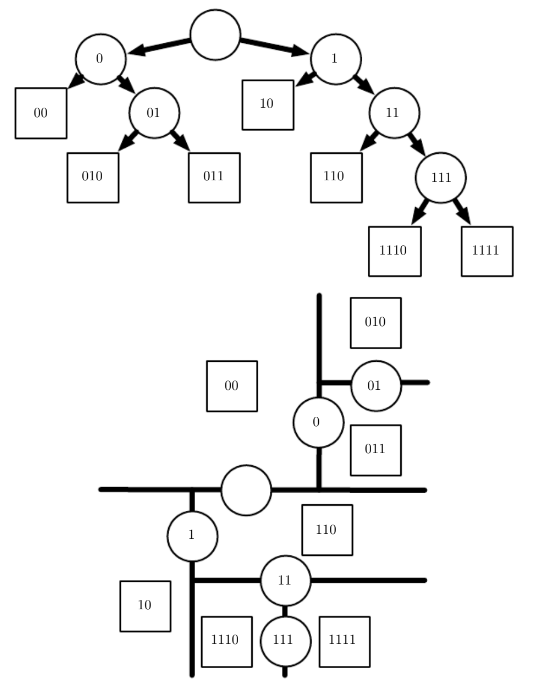
\includegraphics[scale = .7]{IMA/treedesc.png}
\end{center}

Cada nodo del árbol elige enviar el ejemplo de entrada al nodo secundario de la izquierda 
(0) o al nodo secundario de la derecha (1). Los nodos internos se dibujan como círculos y 
los nodos de las hojas como cuadrados. Cada nodo se muestra con un identificador de cadena 
binaria correspondiente a su posición en el árbol, que se obtiene agregando un bit a su 
identificador principal (0=elija izquierda o arriba, 1=elija derecha o abajo). (Abajo) 
El árbol divide el espacio en regiones. \\ 

El plano 2D muestra cómo un árbol de decisión podría 
dividir $\mathbb{R}^{2}$. Los nodos del árbol se trazan en este plano, con cada nodo interno 
dibujado a lo largo de la línea divisoria que utiliza para categorizar ejemplos, y los 
nodos de hoja dibujados en el centro de la región de ejemplos que reciben. El resultado es 
una función constante por partes, con una parte por hoja. Cada hoja requiere al menos un 
ejemplo de entrenamiento para definirse, por lo que no es posible que el árbol de decisión 
aprenda una función que tenga más máximos locales que el número de ejemplos de 
entrenamiento. \cite{Goodfellow-et-al-2016}


% ----------------------------------------------------------------------------------------\
% ---------------------------------------------------------------------------------------\
\subsection{Random Forest}
% ----------------------------------------------------------------------------------------\
% ---------------------------------------------------------------------------------------\

El concepto de sabiduría de la multitud se refiere a la idea de que la respuesta colectiva 
de un grupo de personas al azar a menudo supera la respuesta individual de un experto. 
De manera similar, en el aprendizaje conjunto, al combinar las predicciones de múltiples 
predictores, como clasificadores o regresores, se obtienen predicciones más precisas que 
las de un único predictor. Por lo tanto, el aprendizaje conjunto implica el uso de algoritmos 
que combinan múltiples predictores para mejorar la precisión y la robustez de las predicciones.\\ 

Que significa todo lo de arriba? Los Random Forest (bosques aleatorios) es un algoritmo de 
aprendizaje supervisado que crea un bosque y lo hace de alguna manera aleatorio. Para decirlo 
en palabras simples: el bosque aleatorio crea múltiples árboles de decisión y los combina para 
obtener una predicción más precisa y estable. \cite{Machinelearning}\\

Como ejemplo de método de conjunto, puede entrenar un grupo de clasificadores de árboles de 
decisión, cada uno en un subconjunto aleatorio diferente del conjunto de entrenamiento. 
Luego puede obtener las predicciones de todos los árboles individuales, y la clase que obtiene 
más votos es la predicción del conjunto. Este conjunto de árboles de decisión se denomina 
\textbf{bosque aleatorio} y, a pesar de su simplicidad, es uno de los algoritmos de 
aprendizaje automático más potentes. \cite{géron2022hands}\\ 

Entonces un bosque aleatorio es un conjunto de árboles de decisión, generalmente entrenados 
mediante el método de embolsado, normalmente con $max\_samples$ establecido en el tamaño del 
conjunto de entrenamiento. En lugar de crear un BaggingClassifier y pasarle un 
DecisionTreeClassifier, puede usar la clase \textbf{RandomForestClassifier}, que es más 
conveniente y está optimizada para árboles de decisión (de manera similar, existe una clase 
RandomForestRegressor para tareas de regresión). El siguiente código es un ejemplo de como  
entrena un clasificador de bosque aleatorio con 500 árboles, cada uno limitado a un máximo de 
16 nodos hoja, utilizando todos los núcleos de CPU disponibles:\cite{géron2022hands}\\ 

\begin{lstlisting}[style=mystylepython, language=Python, caption=bosque aleatorio con 500 árboles]
    from sklearn.ensemble import RandomForestClassifier

    rnd_clf = RandomForestClassifier(n_estimators=500, max_leaf_nodes=16, n_jobs=-1, random_state=42)

    rnd_clf.fit(X_train, y_train)

    y_pred_rf = rnd_clf.predict(X_test)    
\end{lstlisting}